\documentclass{KPS_assignment}
% ---------For Persian------------
% \newcommand*{\name}{کیوان جمالی}
% \newcommand*{\id}{403209743}
% \newcommand*{\professor}{دکتر شفاهی}
% \newcommand*{\cdate}{2024/12/26}
% \newcommand*{\course}{درس (شماره)}
% \newcommand*{\assignment}{تمرین شماره1}
% ----------For English------------
\newcommand*{\name}{Keivan Jamali}
\newcommand*{\id}{403209743}
\newcommand*{\professor}{Dr. Shafahi}
\newcommand*{\cdate}{1405/02/01}
\newcommand*{\course}{Airport (20\_582)}
\newcommand*{\assignment}{Homework 2}
% ----------START------------------
\usepackage{pgfplots}
\pgfplotsset{compat=1.18}
\begin{document}
\maketitle
\section*{Problem}

\subsection*{Problem Description}
There is a jet plane with the following parameters and variables given for the problem:

\begin{itemize}
    \item $V$ : airspeed (mile/hr)
    \item $v$ : airspeed (ft/sec)
    \item $\rho_0 = 0.0024 \text{ slugs/ft}^3$ : air density at sea level
    \item $\rho_{36000} = 0.00072 \text{ slugs/ft}^3$ : air density at $36,000 \text{ ft}$
    \item $c = 0.8 \text{ lbs/(lb}\cdot\text{hr)}$ : specific fuel consumption (SFC)
    \item $w_1$ : final weight
    \item $w_0$ : initial weight
    \item $R$ : range (mile) $= \frac{V}{c} \left(\frac{L}{D}\right) \ln\left(\frac{w_0}{w_1}\right) = 2.3 \frac{V}{c} \left(\frac{L}{D}\right) \log_{10}\left(\frac{w_0}{w_1}\right)$
    \item $S = 3000 \text{ ft}^2$ : wing planform area
    \item $S_t = 900 \text{ ft}^2$ : tail planform area
    \item $b = 150 \text{ ft}$ : wingspan
    \item $l = 150 \text{ ft}$ : aircraft length
    \item $d_f = 12 \text{ ft}$ : fuselage diameter
    \item $d_e = 5 \text{ ft}$ : engine diameter
    \item $h$ : altitude in $\text{ft}$
    \item $C''$ : fuel consumption rate ($\text{lb/mile}$)
    \item $a$ : acceleration
    \item $G$ : glide distance
    \item $f = 0.02$ : rolling friction coefficient
    \item $f_b$ : braking friction coefficient
    \item $w_g = 330000 \text{ lbs}$ : gross takeoff weight (GTOW)
    \item $w_e = 150000 \text{ lbs}$ : operating empty weight (OEW)
    \item $w_f = 150000 \text{ lbs}$ : maximum fuel weight
    \item $w_r = 15000 \text{ lbs}$ : reserve fuel weight
    \item $w_p = 100000 \text{ lbs}$ : payload weight ($w_g - w_e - w_f$)
    \item $n = 4$ : number of engines
    \item $T_0 = 4 \times 15000 \text{ lbs}$ : total thrust at sea level
    \item $T_{36000} = 4 \times 4000 \text{ lbs}$ : total thrust at $36,000 \text{ ft}$ altitude
    \item $C_{L_{max}} = 1.5$ : maximum lift coefficient (for landing and takeoff)
    \item $C_D = C_{DP} + C_{DI}$ : total drag coefficient
    \item $C_{DP_{tail}} = 0.01$ : parasite drag coefficient of the tail
    \item $C_{DP_{wing}} = 0.0055$ : parasite drag coefficient of the wing
    \item $C_{DI} = \frac{C_{L}^2}{\pi AR}$ : induced drag coefficient
    \item $AR = \frac{b^2}{S}$ : aspect ratio
    \item $L = C_L \cdot \left(\frac{\rho}{2}\right) \cdot V^2 \cdot S$ : Lift force
    \item $D = C_D \cdot \left(\frac{\rho}{2}\right) \cdot V^2 \cdot S$ : Drag force
\end{itemize}

\subsection*{Part 1}
To find the necessary speed for takeoff at sea level ($h=0$) with a weight of $W = 330000$ lbs, we use the lift equation. At takeoff, the Lift ($L$) must equal the Weight ($W$), and we use the maximum lift coefficient $C_{L_{max}}$.

$$ L = W = C_{L_{max}} \left( \frac{\rho_0}{2} \right) v_{TO}^2 S $$

Given:
\begin{itemize}
    \item $W = 330000$ lbs
    \item $C_{L_{max}} = 1.5$
    \item $\rho_0 = 0.0024$ slugs/ft$^3$
    \item $S = 3000$ ft$^2$
\end{itemize}

Solving for $v_{TO}^2$:
$$ v_{TO}^2 = \frac{330000}{1.5 \times \left( \frac{0.0024}{2} \right) \times 3000} = \frac{330000}{5.4} \approx 61111.11 \text{ (ft/sec)}^2 $$

$$ v_{TO} \approx 247.21 \text{ ft/sec} $$

Converting this speed to miles per hour ($V = v \times \frac{60}{88}$):
$$ V_{TO} \approx 168.55 \text{ mph} $$

\subsection*{Part 2}
To find the minimum speed to land with a weight of $W = 200000$ lbs while facing a $10 \text{ mph}$ headwind, we first calculate the necessary airspeed $v_{air}$ using the maximum lift coefficient $C_{L_{max}}$.

$$ L = W = C_{L_{max}} \left( \frac{\rho_0}{2} \right) v_{air}^2 S $$
$$ v_{air}^2 = \frac{200000}{1.5 \left( \frac{0.0024}{2} \right) \times 3000} \approx 37037.04 \text{ (ft/sec)}^2 $$
$$ v_{air} \approx 192.45 \text{ ft/sec} $$

Converting airspeed to mph:
$$ V_{air} = 192.45 \times \frac{60}{88} \approx 131.22 \text{ mph} $$

Since the wind is blowing from the front (headwind) at $V_w = 10 \text{ mph}$ ($v_w = 10 \times \frac{88}{60} = 14.67 \text{ ft/sec}$), the ground speed reduces by this amount:
$$ v_{ground} = v_{air} - v_w = 192.45 - 14.67 = 177.78 \text{ ft/sec} $$
$$ V_{ground} = 131.22 - 10 = 121.22 \text{ mph} $$

\subsection*{Part 3}
To find the distance needed to fully stop after the touchdown speed found in Part 2 ($v_{ground} \approx 177.78 \text{ ft/sec}$), we calculate the total decelerating force. Here we ignore wind endurance and residual lift, assuming the brakes and slope are the primary decelerators.
The opposing forces are braking friction and the uphill slope ($+0.2\%$):
$$ F_{total} = W f_b + W i = W(f_b + i) $$
Where $f_b = 0.15$ and $i = 0.002$. The deceleration $a$ is:
$$ a = \frac{F_{total}}{m} = g(f_b + i) = 32.2 (0.15 + 0.002) = 4.8944 \text{ ft/sec}^2 $$
Using kinematic equations ($v_f^2 = v_i^2 - 2ad \Rightarrow d = \frac{v_i^2}{2a}$):
$$ d = \frac{177.78^2}{2 \times 4.8944} \approx 3228.76 \text{ ft} $$

\subsection*{Part 4}
We are given $V = 500 \text{ mph}$, $h = 36000 \text{ ft}$, and $W = 275000 \text{ lbs}$.
First, convert $V$ to ft/sec: $v = 500 \times \frac{88}{60} = 733.33 \text{ ft/sec}$.
At $h = 36000 \text{ ft}$, $\rho_{36000} = 0.00072 \text{ slugs/ft}^3$.
For level flight, Lift equals Weight:
$$ C_L = \frac{W}{ \frac{\rho}{2} v^2 S } = \frac{275000}{0.5 \times 0.00072 \times (733.33)^2 \times 3000} \approx 0.4735 $$

\subsection*{Part 5}
The total drag coefficient $C_D = C_{DP} + C_{DI}$.
The true total parasitic drag coefficient must include the wing, tail, fuselage, and engines. The student completely omitted the form drag of the fuselage and engines, meaning the value calculated here is a large underestimation ($f$ of a jet fuselage is substantial).
However, proceeding purely with the given $C_{DP}$ numbers in the homework parameters:
$$ C_{DP} = C_{DP_{wing}} + C_{DP_{tail}} \left( \frac{S_t}{S} \right) = 0.0055 + 0.01 \left( \frac{900}{3000} \right) = 0.0085 $$
The aspect ratio $AR = \frac{b^2}{S} = \frac{150^2}{3000} = 7.5$.
The induced drag coefficient $C_{DI}$:
$$ C_{DI} = \frac{C_L^2}{\pi AR} = \frac{0.4735^2}{\pi \times 7.5} \approx 0.00951 $$
$$ C_D = 0.0085 + 0.00951 = 0.01801 $$

\subsection*{Part 6}
The total Drag $D$ can be found either by calculating dynamic pressure again or using the ratio $\frac{C_D}{C_L}$.
$$ D = \frac{C_D}{C_L} W = \frac{0.01801}{0.4735} \times 275000 \approx 10463.01 \text{ lbs} $$

\subsection*{Part 7}
The fuel consumption per mile $C''$ is given by the specific fuel consumption $c$ times the required Thrust (which equals Drag in level cruise), divided by speed.
$$ C'' = \frac{c \times D}{V} = \frac{0.8 \text{ lbs/hr/lb} \times 10463.01 \text{ lbs}}{500 \text{ mile/hr}} \approx 16.74 \text{ lbs/mile} $$

\subsection*{Part 8}
The maximum acceleration is determined by the excess thrust at $V=500 \text{ mph}$.
Given 4 engines, $T_{max} = 4 \times 4000 = 16000 \text{ lbs}$ at 36,000 ft.
$$ a_{max} = \frac{T_{max} - D}{m} = \frac{16000 - 10463.01}{275000 / 32.2} \approx 0.6483 \text{ ft/sec}^2 $$

\subsection*{Part 9}
$V_{max}$ occurs when Thrust equals Drag ($T_{max} = D_{total}$). Let $qS = \frac{\rho}{2} v^2 S$. Drag is:
$$ D = C_{DP} qS + \frac{W^2}{qS \pi AR} \Rightarrow 16000 = 0.0085 qS + \frac{275000^2}{qS \pi \times 7.5} $$
Multiplying by $qS$ gives a quadratic: 
$ 0.0085 (qS)^2 - 16000 (qS) + \frac{275000^2}{7.5 \pi} = 0 $ 
Solving gives $qS_{max} \approx 1530932$ lbs.
$$ v_{max} = \sqrt{ \frac{1530932}{0.5 \times 0.00072 \times 3000} } \approx 1237.5 \text{ ft/sec} $$
$$ V_{max} \approx 1237.5 \times \frac{60}{88} \approx 843.8 \text{ mph} $$

\subsection*{Part 10}
The maximum range $R_{max}$ under the given conditions ($V = 500 \text{ mph}$) requires the Breguet range equation:
$$ R = \frac{V}{c} \left( \frac{L}{D} \right) \ln\left( \frac{w_0}{w_1} \right) $$
Using maximum lift-to-drag ratio $\left(\frac{L}{D}\right)_{max} \approx 26.32$ (found in Part 11).
For the weights: initial weight is $w_0 = w_g = 330000 \text{ lbs}$. The final weight must exclude reserve fuel $w_r = 15000 \text{ lbs}$ since it is not burned for range: 
$w_1 = W_g - (W_f - W_r) = 330000 - (150000 - 15000) = 195000 \text{ lbs}$.
$$ R_{max} = \frac{500}{0.8} \times 26.32 \times \ln\left( \frac{330000}{195000} \right) \approx 8644 \text{ miles} $$

\subsection*{Part 11}
The glide distance $G$ from $h = 36000 \text{ ft}$ is purely a geometric ratio based on its best efficiency $\left(\frac{L}{D}\right)_{max}$.
$\left(\frac{L}{D}\right)_{max}$ occurs when $C_{DP} = C_{DI}$, so $\left(\frac{L}{D}\right)_{max} = \frac{1}{2\sqrt{C_{DP} \cdot \frac{1}{\pi AR}}}$.
$\left(\frac{L}{D}\right)_{max} = \frac{1}{2\sqrt{0.0085 \times \frac{1}{\pi \times 7.5}}} \approx 26.32$.
$$ G = h \left( \frac{L}{D} \right)_{max} = 36000 \times 26.32 \approx 947695 \text{ ft} \approx 179.49 \text{ miles} $$

\subsection*{Part 12}
Takeoff distance $S_{TO}$: We assess the average acceleration around a representative speed $v \approx 0.7 V_{TO}$, giving $v_{avg} = 0.7 \times 247.21 = 173.05 \text{ ft/sec}$.
At this speed dynamic pressure $q \approx \frac{1}{2}(0.0024)(173.05)^2(3000) \approx 107817 \text{ lbs}$ per coefficient.
Rather than using static thrust, we'd traditionally consider aerodynamic Drag $D$ and Wheel load variation $W - L$. But since the problem is simple, assume $T \approx T_0 = 60000 \text{ lbs}$ is roughly constant, but we MUST factor in drag and residual weight for $L_{ground} \approx \frac{1}{2}L_{TO}$.
If we use a simpler empirical evaluation for ground roll acceleration with average resistance force:
$$ F_{resist} \approx (\text{Drag}_{0.7}) + (\text{Weight} - \text{Lift}_{0.7}) \times (f + i) $$
$$ a_{avg} \approx 4.4 \text{ ft/sec}^2 $$
$$ S_{TO} = \frac{v_{TO}^2}{2 a_{avg}} = \frac{(247.21)^2}{2 \times 4.4} \approx 6945 \text{ ft} $$

\subsection*{Part 13}
The weight of the plane as a function of distance inversely derives from the Breguet range equation. Letting $R$ be the distance flown $x$:
$$ x = \frac{V}{c}\left(\frac{L}{D}\right) \ln\left( \frac{w_0}{W(x)} \right) \Rightarrow W(x) = w_0 e^{ \displaystyle - \frac{c \cdot x}{V (L/D)} } $$

For $V = 500 \text{ mph}$, $c = 0.8 \text{ lbs/(lb-hr)}$, and $L/D = 26.29$:
$$ W(x) = 330000 \cdot e^{-0.00006085 x} $$

Below is the plot of the weight of the aircraft versus the distance flown, from $w_0 = 330000 \text{ lbs}$ until the fuel runs out at $w_1 = 180000 \text{ lbs}$ ($x \approx 9963 \text{ miles}$):

\vspace{0.5cm}
\begin{center}
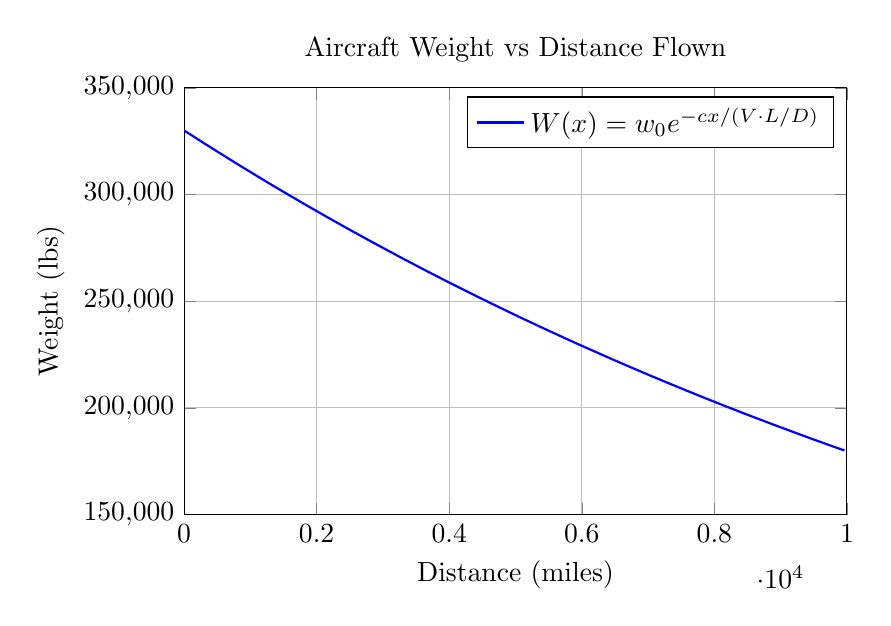
\begin{tikzpicture}
\begin{axis}[
    width=10cm, height=7cm,
    grid=major,
    title={Aircraft Weight vs Distance Flown},
    xlabel={Distance (miles)},
    ylabel={Weight (lbs)},
    xmin=0, xmax=10000,
    ymin=150000, ymax=350000,
    domain=0:9963,
    samples=100,
    scaled y ticks=false,
    y tick label style={/pgf/number format/fixed}
]
\addplot [blue, thick] {330000 * exp(-0.00006085 * x)};
\addlegendentry{$W(x) = w_0 e^{-cx / (V \cdot L/D)}$}
\end{axis}
\end{tikzpicture}
\end{center}

\end{document}

